\documentclass{article}
\usepackage{amsmath}
\usepackage{graphicx}
\usepackage{algorithm}
\usepackage{algorithmic}
\newcommand{\dastates}{\underline{\textbf{States}}}
\newcommand{\daonreceive}{\underline{\textbf{On receive}}\ }
\newcommand{\dasend}{\textbf{Send}\ }
\newcommand{\tinsert}{\textbf{Insert}\ }
\newcommand{\tdelete}{\textbf{Delete}\ }
\newcommand{\tupdate}{\textbf{Update}\ }
\newcommand{\daonupdate}{\underline{\textbf{On update to}}\ }
\newcommand{\daperiodic}{\underline{\textbf{At each period}}\ }
\newcommand{\daonstate}{\underline{\textbf{On reaching state}}\ }
\newcommand{\daon}{\underline{\textbf{On}}\ }
\newcommand{\AND}{$\wedge$\ }
\newcommand{\NOT}{$\neg$\ }
\newcommand{\OR}{$\vee$\ }

\newtheorem{theorem}{Theorem}[section]
\newtheorem{lemma}[theorem]{Lemma}
\newtheorem{proposition}[theorem]{Proposition}
\newtheorem{corollary}[theorem]{Corollary}
\newtheorem{fact}[theorem]{Fact}
\newtheorem{definition}[theorem]{Definition}


\graphicspath{ {figures/}}
\bibliographystyle{plain}
\usepackage{cite}

\title{Causal Consistency??}
\author{Yu-En Lu \\University of Cambridge \and Petros Maniatis \\Intel Research Berkeley}
\date{$Id: full.tex,v 1.1 2007/01/18 18:18:55 ericyu Exp $}

\begin{document}
\maketitle

\section{Single Site, Single Event Atomicity}
\begin{definition}[Causal Consistency]
	mmm, not quite clear here yet.
\end{definition}

\begin{definition}[Single Event Atomicity]
	A dataflow is said to have single event atomicity if
	ALL derived events and actions as a result of an event 
	are seen by all subsequent events.
\end{definition}

\begin{verbatim}
materialize(tBuf,infinity,infinity,keys(2,3,5)).
b1 delete tBuf(@X,Y,FID,PKT,S) :- ack(@X,Y,FID,L,R), tBuf(@X,Y,FID,PKT,S), S <= L.

b2 bufMon(@X,Y,FID,count<*>) :- tBuf(@X,Y,FID,PKT,S).

b3 doX(@X,Y,FID) :- bufMon(@X,Y,FID,C), C == 5.
\end{verbatim}

The following code is the current event loop which fires timer callbacks and network I/O call backs
at each iteration.
\begin{verbatim}
while(1){
     timer_call_back();
     file_descriptor_call_back();
}
\end{verbatim}


\begin{figure}[h]
	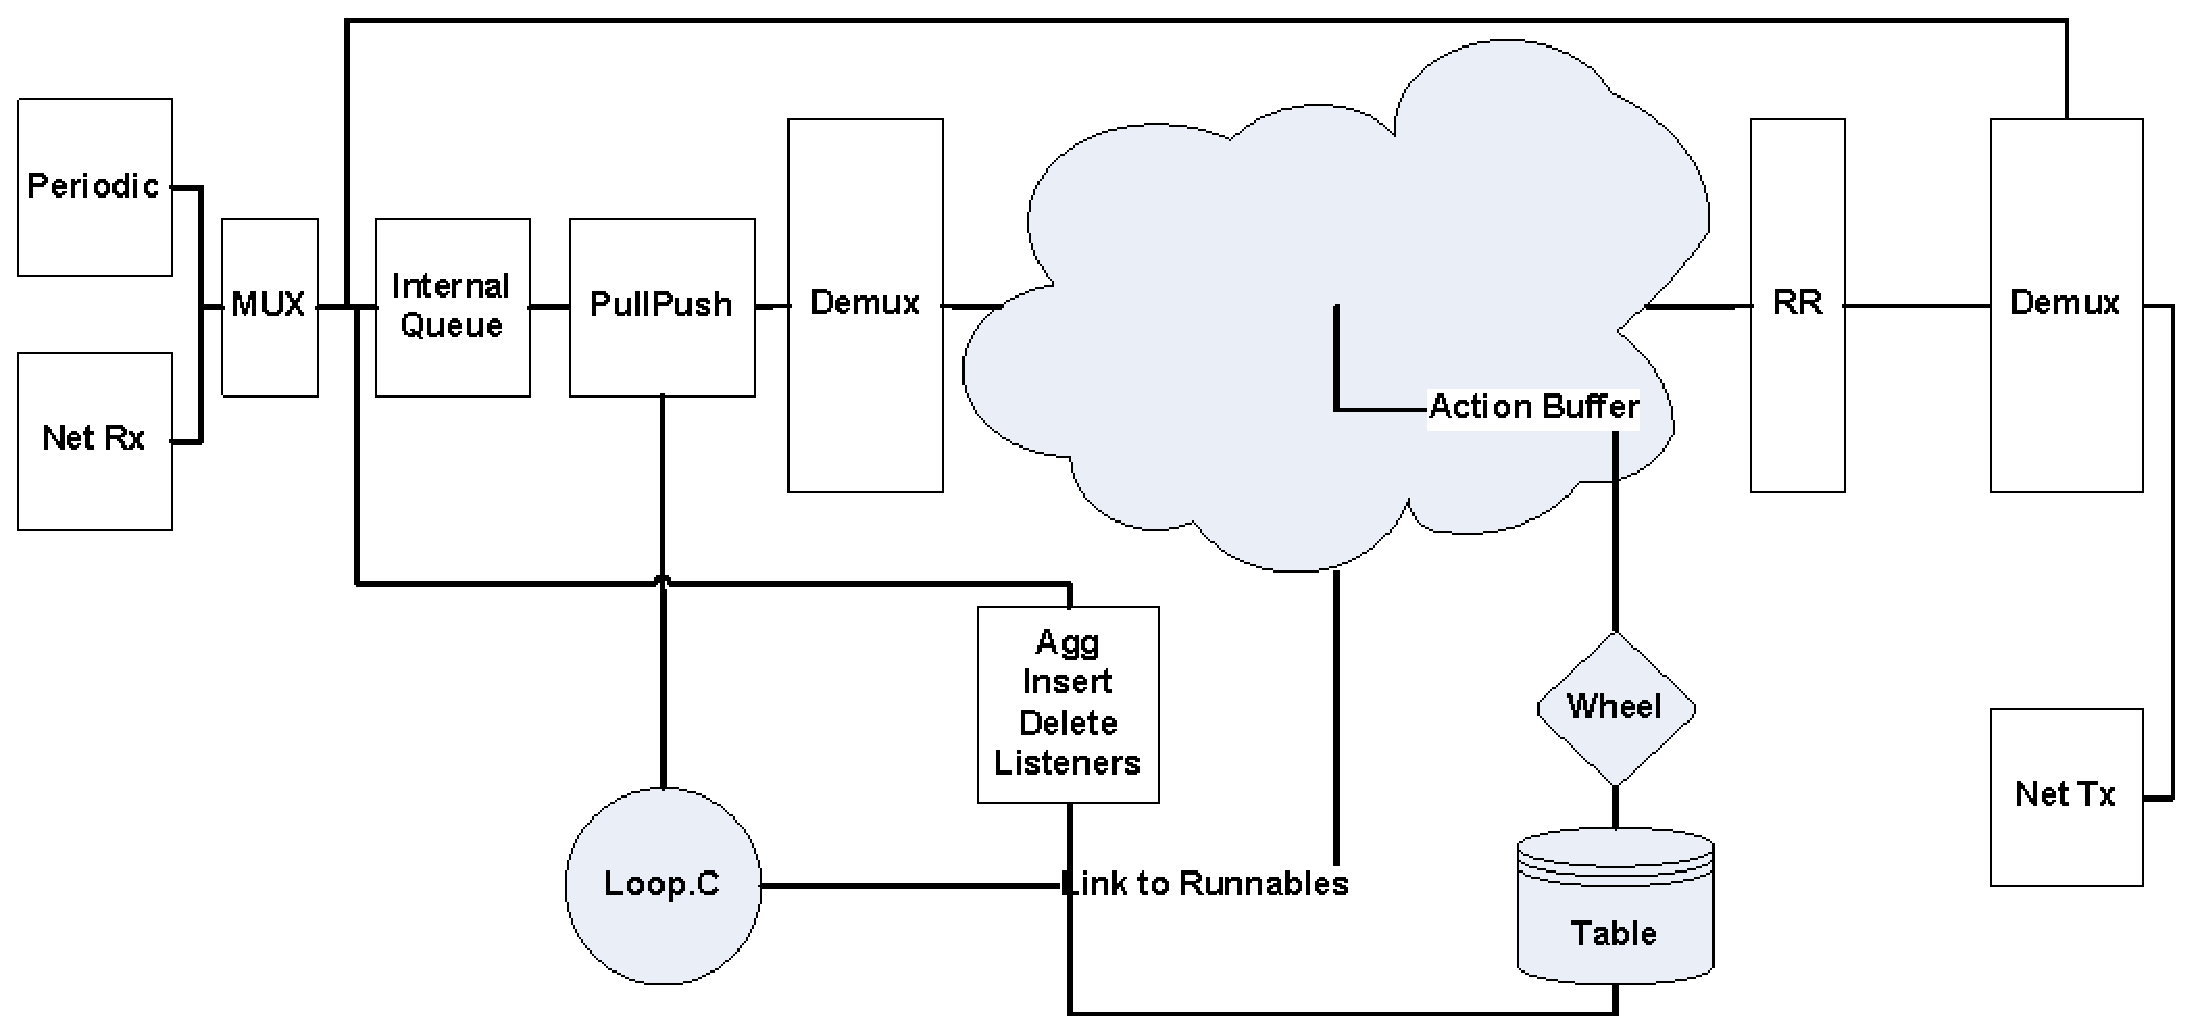
\includegraphics[width=10cm]{SSSingleEventAtomicityDF.eps}
	\caption{Dataflow for proposed single site, single event atomicity semantics.}
	\label{fig:SSSingleEventAtomicityDF}
\end{figure}



\begin{algorithm}[h]
	\begin{algorithmic}
		\WHILE{1}
			\STATE Move an event $e$ into inner queue
			\WHILE{ inner queue is not empty}
				\STATE Push an event from inner queue to demux
				\WHILE{$\exists$ runnable R in DAG}
					\STATE Run R
				\ENDWHILE
				\STATE Turn the wheel of time (Apply the insertion and deletion)
			\ENDWHILE
		\ENDWHILE
	\end{algorithmic}
	\caption{Proposed algorithm for single site, single event atomicity}
	\label{alg:SSAtomicity}
\end{algorithm}

We should be able to implement algorithm \ref{alg:SSAtomicity} 
by the following pseudo code in loop.C.

\begin{verbatim}
while(1){
     timer_call_back();
     file_descriptor_call_back();
     inner_queue_pull(); //this is actually implemented by invoking pull explicitly
     inner_queue_block_external_ports();
     while(!inner_queue.empty()){
        inner_queue_pp_pull();
        while(!runnables.empty()){ //this is to be done through IRunnable interface
              runnables.top().run();
        }
        wheel.turn();//appy the actual add/delete action
     }
     inner_queue_unblock_external_ports();
}
\end{verbatim}

Assumptions:
\begin{itemize}
	\item There is a notion where periodic is either idempotent or not
	\item Aggregation objects are calculated immediately when the table is updated
	\item Facts are implemented as initial tuples in the external queue (will check with Tyson)
\end{itemize}

Requirements:
\begin{itemize}
	\item Internal queue must be able to block certain input ports (controlled by loop.C)
	\item Internal queue and the network queue element must be infinite (at least in theory)
		in order to have single event atomicity
\end{itemize}


Modification high lights in figure \ref{fig:SSSingleEventAtomicityDF}:
\begin{itemize}
	\item Change the insert/delete element to send msg to the wheel element instead
	\item Have all new pullpush elements to register its state with the singleton object, runnables.
	\item All insert/delete listener elements should be linked to the internal queue, and should be
		invoked immediately when the table is updated
	\item 0-lifetime Tuples (events) coming out of the RR element are now routed directly to
		internal queue
	\item loop.C would call pullpush of internal queue after all runnables are quiencene. 
\end{itemize}

\bibliography{mapreduce}
\end{document}
